The IP-shuffle script offers a systematic approach to dynamic IP address assignment for network interfaces in Linux and FreeBSD environments. Built around Bash scripting, it seamlessly orchestrates the IP address allocation process. By default, the program runs every 3 minutes, based on the provided cronjob. During execution, the script dynamically configures the IP address, gateway, network interface details, and other parameters, providing a flexible framework for network configuration. Through dedicated functions such as
\begin{verbatim}
generate_random_ip (), 
check_ip_availability(), 
and validate_network_config(), 
\end{verbatim}
the script ensures that the assigned IP addresses are compatible with the network infrastructure. It also incorporates error-trapping mechanisms and support for common Unix signals to enhance reliability and resilience, safeguarding against potential errors or interruptions. The script's flexibility is maintained through adherence to modular design principles, allowing seamless adaptation to diverse network configurations and environments. However, since the IP addresses are not persistent after a reboot for DHCP-configured machines, the script includes functions like \texttt{reset\_network()} for error recovery. The IP-shuffle script encapsulates a robust solution for automating network interface configuration tasks, embodying a sophisticated yet accessible approach to dynamic IP address management.

\label{sec:figs}
%-------------------------------------------------------------------------------
%---------------------------


\begin{figure}
 \caption{Network Topology Diagram}
  \centering
   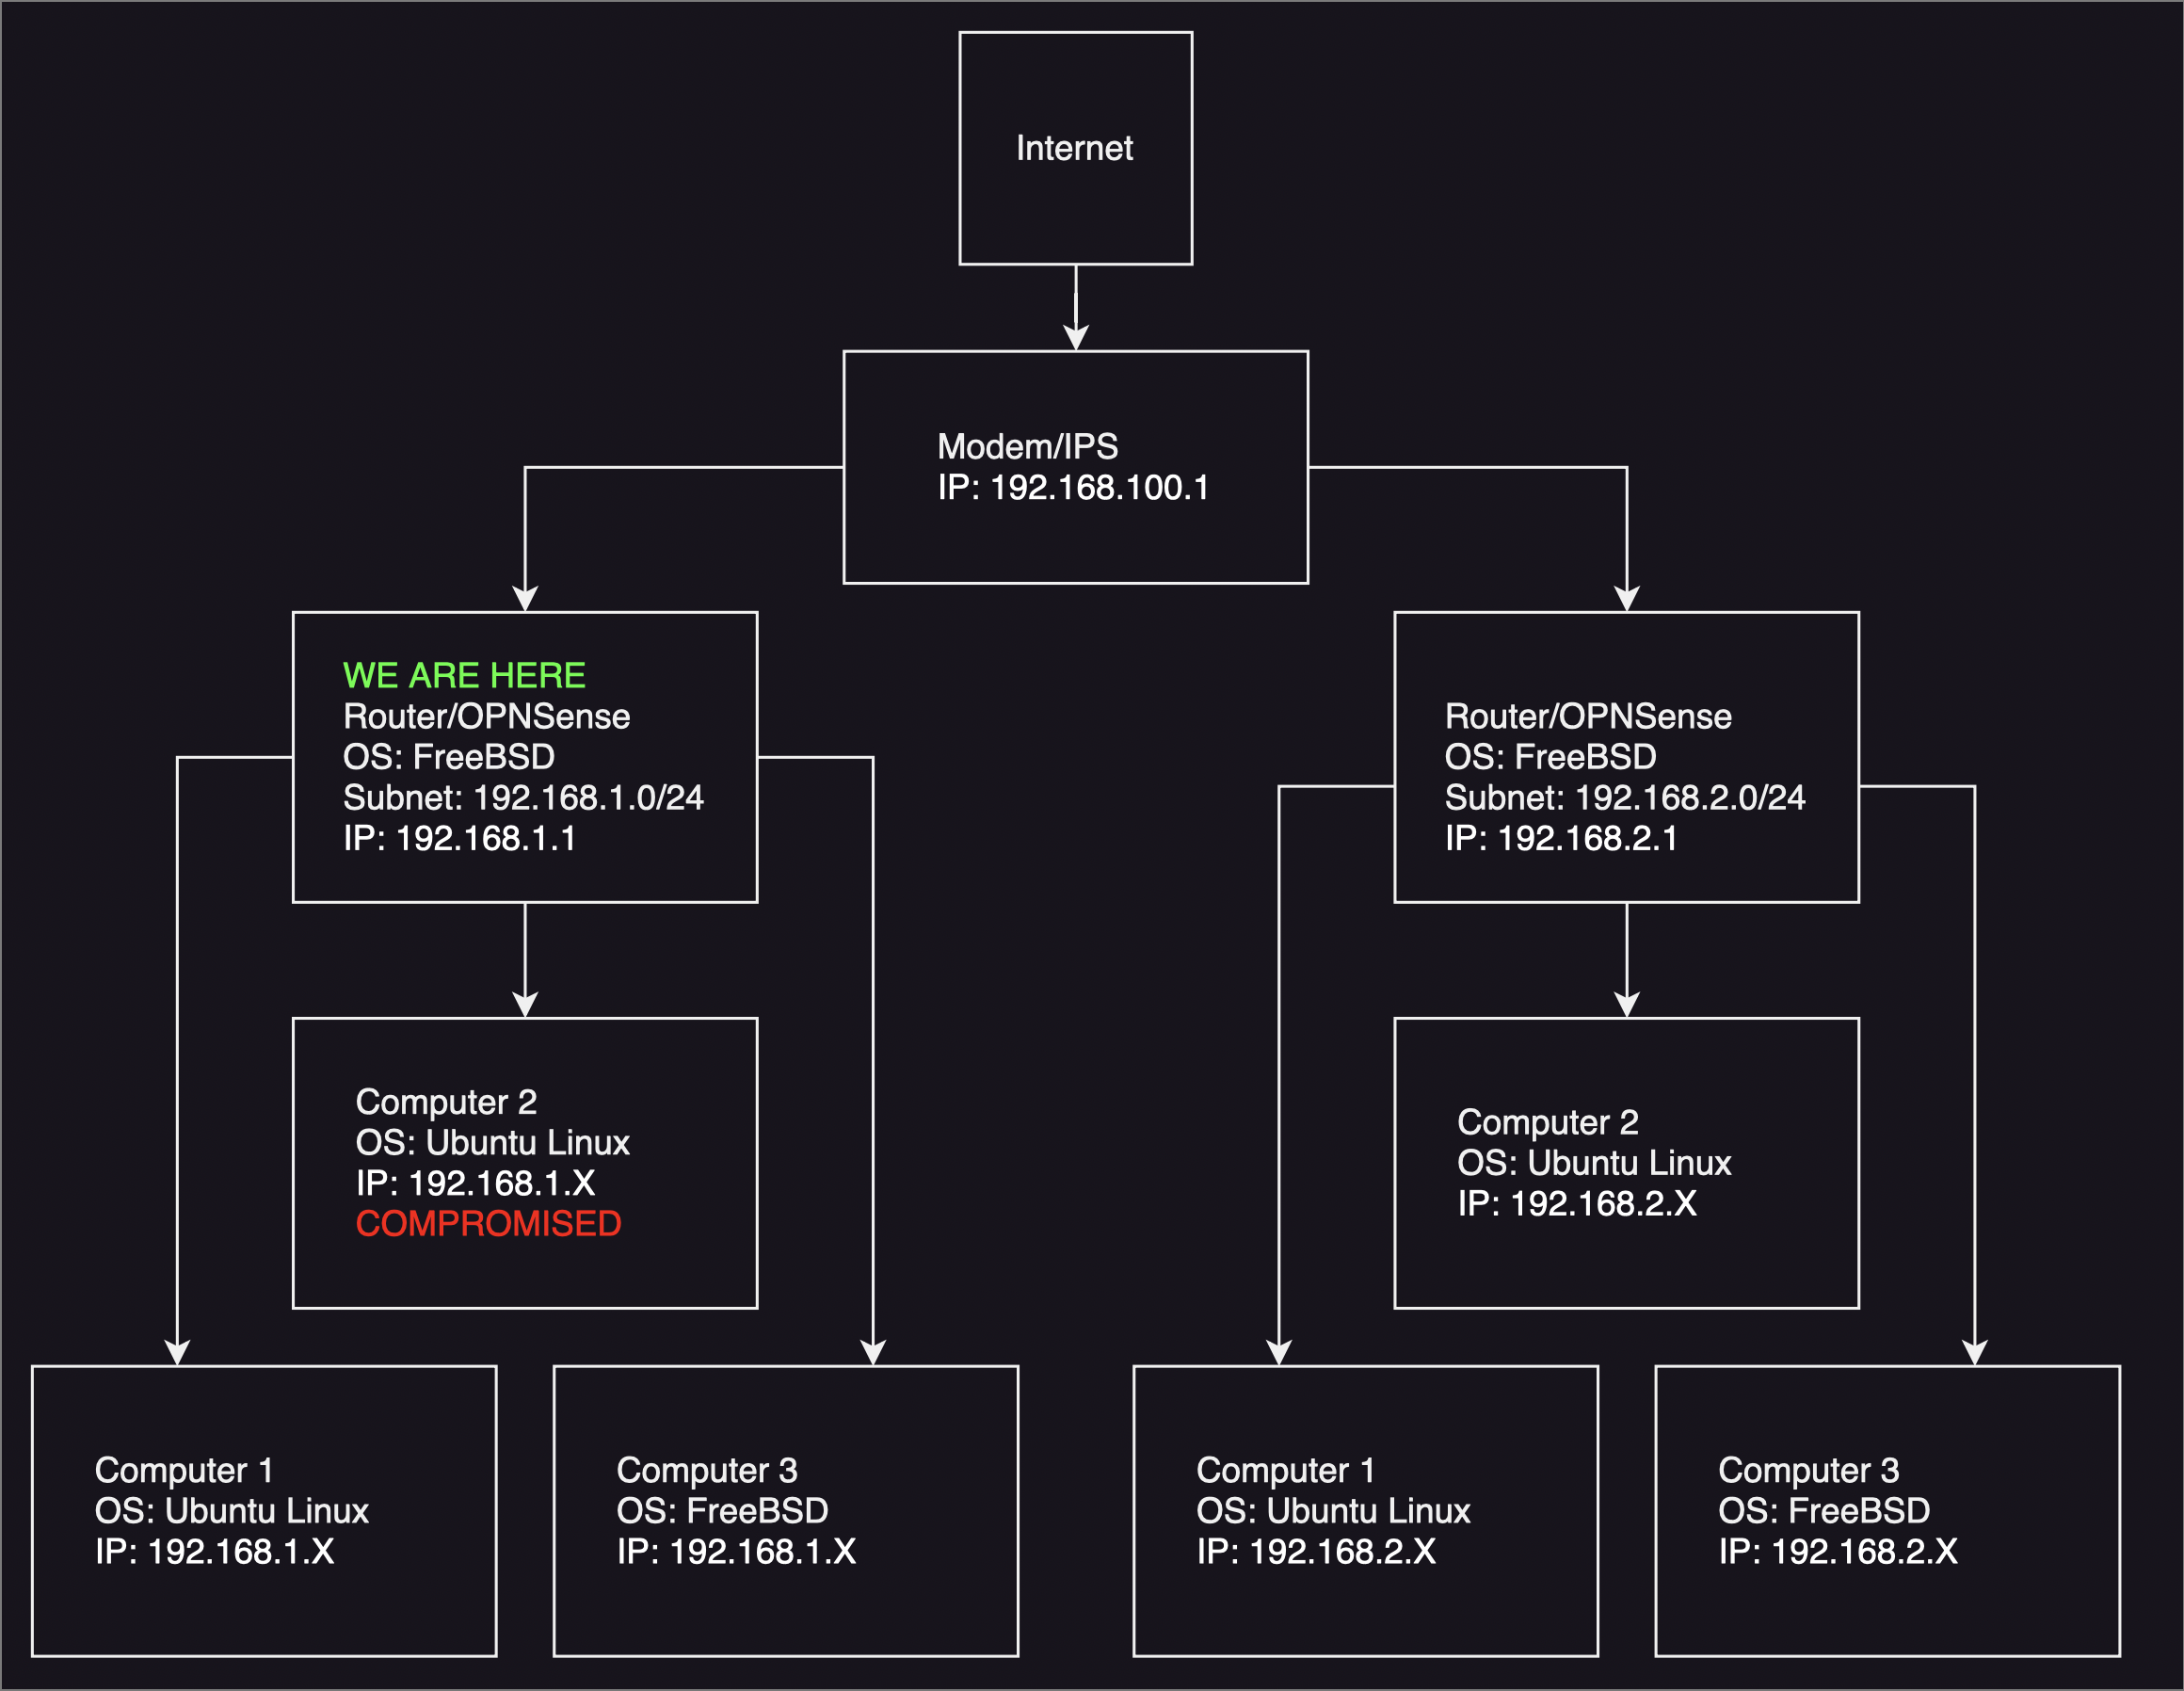
\includegraphics[width=0.5\textwidth]{diagram.png}
\end{figure}

%% %---------------------------
 




